\chapter{The mesh}

\devnote{This chapter is currently being written\ldots}

% FIXME: Triangular, tetrahedral, include some images,
% FIXME: mesh refinement, connectivity, iterators, file formats, local
% FIXME: ordering

The concept of a \emph{mesh} is central in the implementation of
adaptive Galerkin finite element methods for partial differential equations.
Related important concepts include \emph{vertices}, \emph{cells},
\emph{edges}, \emph{faces}, \emph{boundaries}, and \emph{mesh hierarchies}. These 
concepts are all implemented as C++ classes in \dolfin{}, as shown in Figure \ref{fig:meshclasses}.

\begin{figure}[htbp]
  \begin{center}
    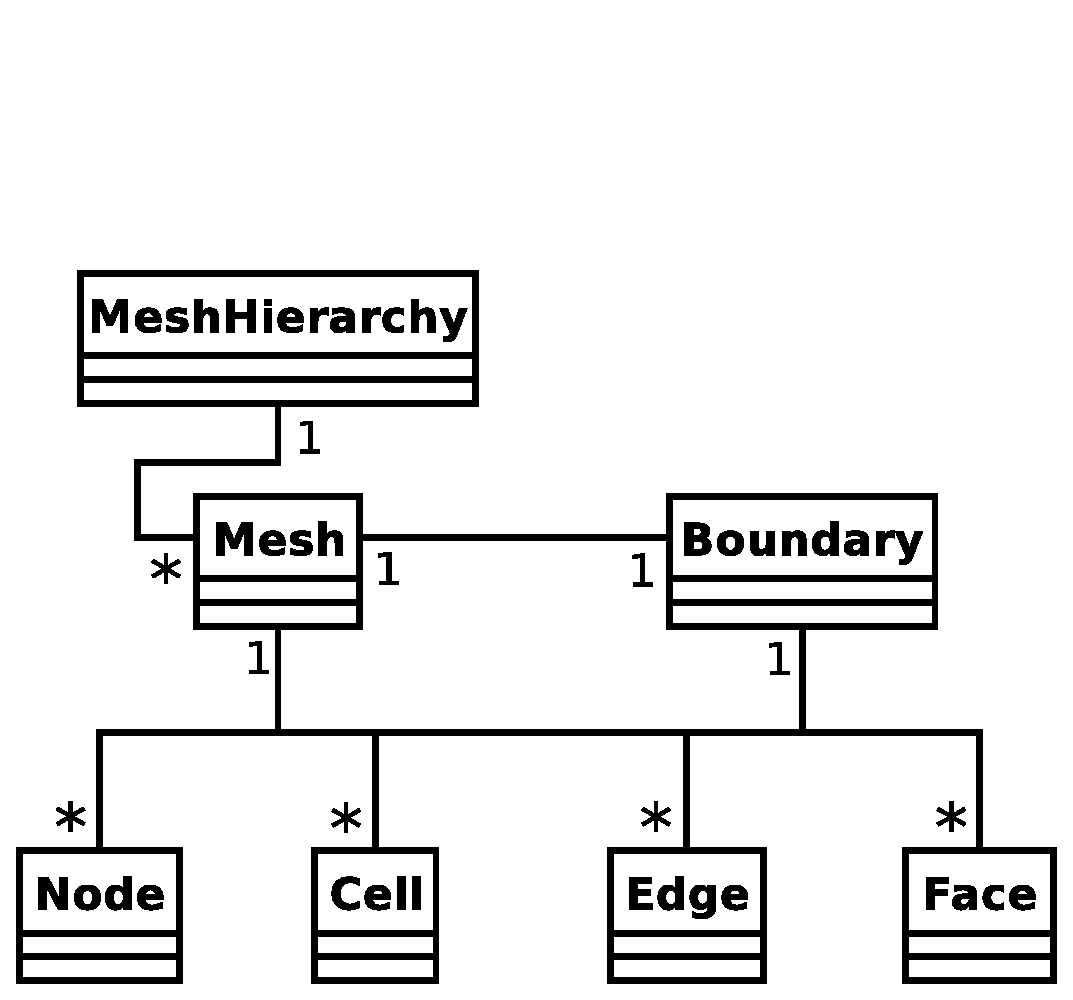
\includegraphics[width=10cm]{eps/mesh-components.eps}
    \caption{Class diagram of the basic mesh classes in \dolfin{}.}
    \label{fig:meshclasses}
  \end{center}
\end{figure}

\section{Mesh iterators}

Algorithms operating on a mesh, including adaptive mesh refinement,
can often be expressed in terms of
\emph{iterators}, i.e., objects used for the traversal of aggregate
structures, such as the list of vertices contained in a mesh. Iterators
implemented in \dolfin{} include a \texttt{VertexIterator},
\texttt{CellIterator}, \texttt{Edge}\-\texttt{Iterator}, \texttt{FaceIterator},
and a \texttt{MeshIterator}. The following code illustrates how to
iterate over all vertex neighbors of all vertices of all cells within a
given mesh:
\begin{code}
  for (CellIterator c(m); !c.end(); ++c)
    for (VertexIterator v1(c); !v1.end(); ++v1)
      for (VertexIterator v2(n1); !v2.end(); ++v2)
        cout << *v2 << endl;
\end{code}

\section{Mesh refinement}

Adaptive mesh refinement is implemented in \dolfin{} for triangular
meshes (in 2D) and tetrahedral meshes (in 3D), see Figure
\ref{fig:refinedmeshes}, based on the algorithm given in \cite{Bey95}.
To refine a mesh, the cells (triangles or tetrahedrons) are first
marked according to some criterion for refinement, before the mesh is
refined. A hierarchy of meshes, that can be used for example in a
multigrid computation, is automatically created.

\begin{figure}
  \begin{center}
    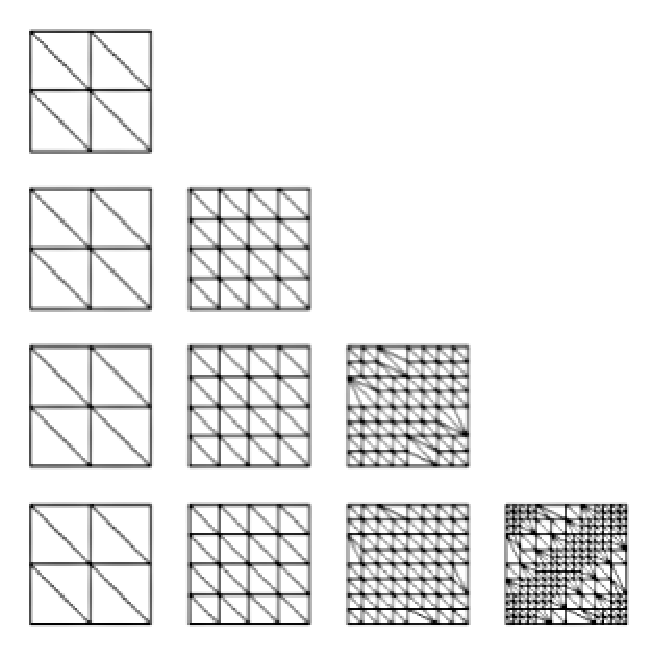
\includegraphics[width=6cm]{eps/mesh2d.eps}
    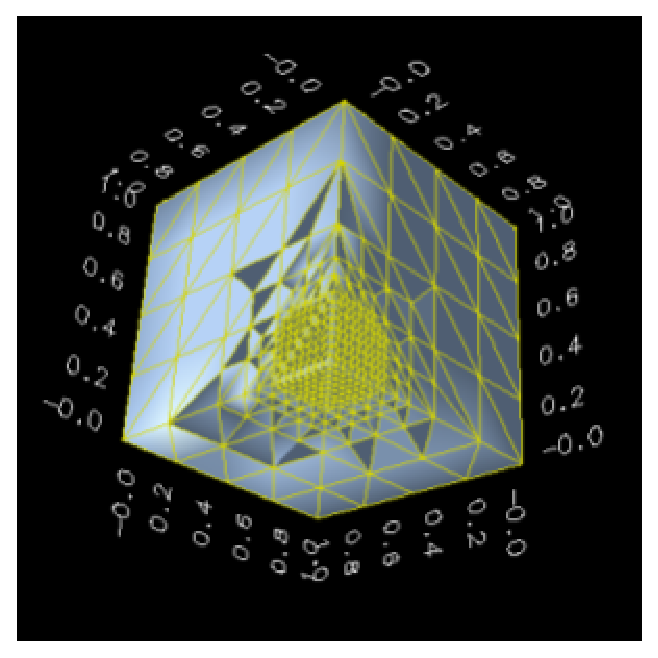
\includegraphics[width=6cm]{eps/mesh3d.eps}
    \caption{Adaptive mesh refinement of triangular and tetrahedral meshes in \dolfin{}.}
    \label{fig:refinedmeshes} 
  \end{center}
\end{figure}

The following example illustrates how to iterate over the \texttt{Cell}s of
a \texttt{Mesh} to mark some \texttt{Cell}s for refinement, before refining
the \texttt{Mesh}:
\begin{code}
  // Mark cells for refinement
  for (CellIterator cell(mesh); !cell.end(); ++cell)
    if ( ... )
      cell->mark();

  // Refine mesh
  mesh.refine();
\end{code}

It is also possible to directly mark all \texttt{Cell}s for refinement
to refine the \texttt{Mesh} uniformly:
\begin{code}
  // Refine all cells
  mesh.refineUniformly();
\end{code}
